\documentclass[twoside]{article}

\usepackage{amsmath}
\usepackage{amsfonts}
\usepackage{graphicx}
\usepackage{multirow}
\usepackage{fontspec}
\usepackage{hyperref}
\usepackage{xepersian}
% Font Settings ======================
\setlatintextfont{LinLibertine}[Path = fonts/latin/]
\settextfont{HMXKayhan}[
Path = fonts/fa/ ,
BoldFont = HMXKayhanBd]
% Graphic Settings ===================
\graphicspath{{images/}}
\DeclareGraphicsExtensions{.jpeg,.png,.jpg}


\title{\Huge پیش گزارش آزمایش 6 آز مدار منطقی }
\author{\Large علی دهقانی ، ماهان بیهقی}
\date{دانشگاه صنعتی شریف}

\begin{document}
	\maketitle
	\newpage
	\section*{نام آزمایش}
	تایمر ماشین لباسشویی
	
	\section*{اهداف آزمایش}
	پیاده سازی یک یک تایمر برای ماشین لباسشویی
	
	\section*{شرح آزمایش}
	
	\subsection*{لیست تراشه ها و قطعات مورد نیاز} 
	\begin{itemize}
		\item
		\href{https://datasheetspdf.com/pdf-file/248168/STMicroelectronics/74192/1}{74192 SYNCHRONOUS 4-BIT UP/DOWN COUNTER}
		\item
		\href{https://www.esi.uclm.es/www/isanchez/apuntes/ci/74151.pdf}{74151 MULTIPLEXER}
		\item
		\href{https://www.ti.com/lit/ds/symlink/sn74ls138.pdf}{74138 DECODER/DEMULTIPLEXER}
		\item
		\href{https://www.rhydolabz.com/documents/74LS48.pdf}{7448 SEVEN-SEGMENT DECODER}
	\end{itemize}
	
	\subsection*{شرح آزمایش}
	این ماشین لباسشویی دو برنامه شستشو با آب گرم و آب سرد دارد که با تغییر وضعیت کلید مشخص میشود. 
	
	در برنامه شستشو با آب سرد به ترتیب مراحل آبگیری ، شستشو ، تخلیه و سپس خشک کردن در مدت زمان 2 و 3 و 2 و 2 پالس ساعت انجام میشود.
	
	در برنامه شستشو با آب گرم به ترتیب مراحل آبگیری ، گرم کردن آب ، شستشو ، تخلیه و خشک کردن در مدت زمان 2 و 3 و 3 و 2 و 2 پالس ساعت انجام میشود.
	
	با زدن کلید کار ماشین لباس شویی شروع میشود ، به شرط آنکه شیر آب باز و در ماشین لباس شویی بسته باشد و برنامه مورد نظر انتخاب شده باشد.
	
	سیگنال های ورودی مدار : کلید شروع ، باز و بسته بودن شیر آب ، باز و بسته بودن در ماشین ، انتخاب عملیات آب سرد یا گرم
	
	سیگنال های خروجی مدار : شستشو ، گرم کردن آب ، عملیات آبگیری ، تخلیه و خشک کردن
	

	
	\subsection*{مراحل آزمایش و مدارات}
	از تراشه 74192 برای تغییر کلاک به 2 یا 3 پالس ساعت استفاده میکنیم. طبق دیتاشیت این تراشه ، پایه های D0 تا D3 را به اندازه کلاک مورد نظر اندازه دهی میکنیم و خروجی های آن ها را به مالتی پلکسر ها وصل میکنیم. این 4 مالتی پلکسر به عنوان ورودی کانتر معکوس استفاده میشوند که تعیین میکند عملیات چند پالس طول بکشد. با 0 شدن این کانتر عملیات بعدی آغاز میشود.
	
	البته مدار انتخابگر عملیات در مدار پیشنهادی کامل نیست.
	
	\begin{figure}[h!]
		\begin{center}
			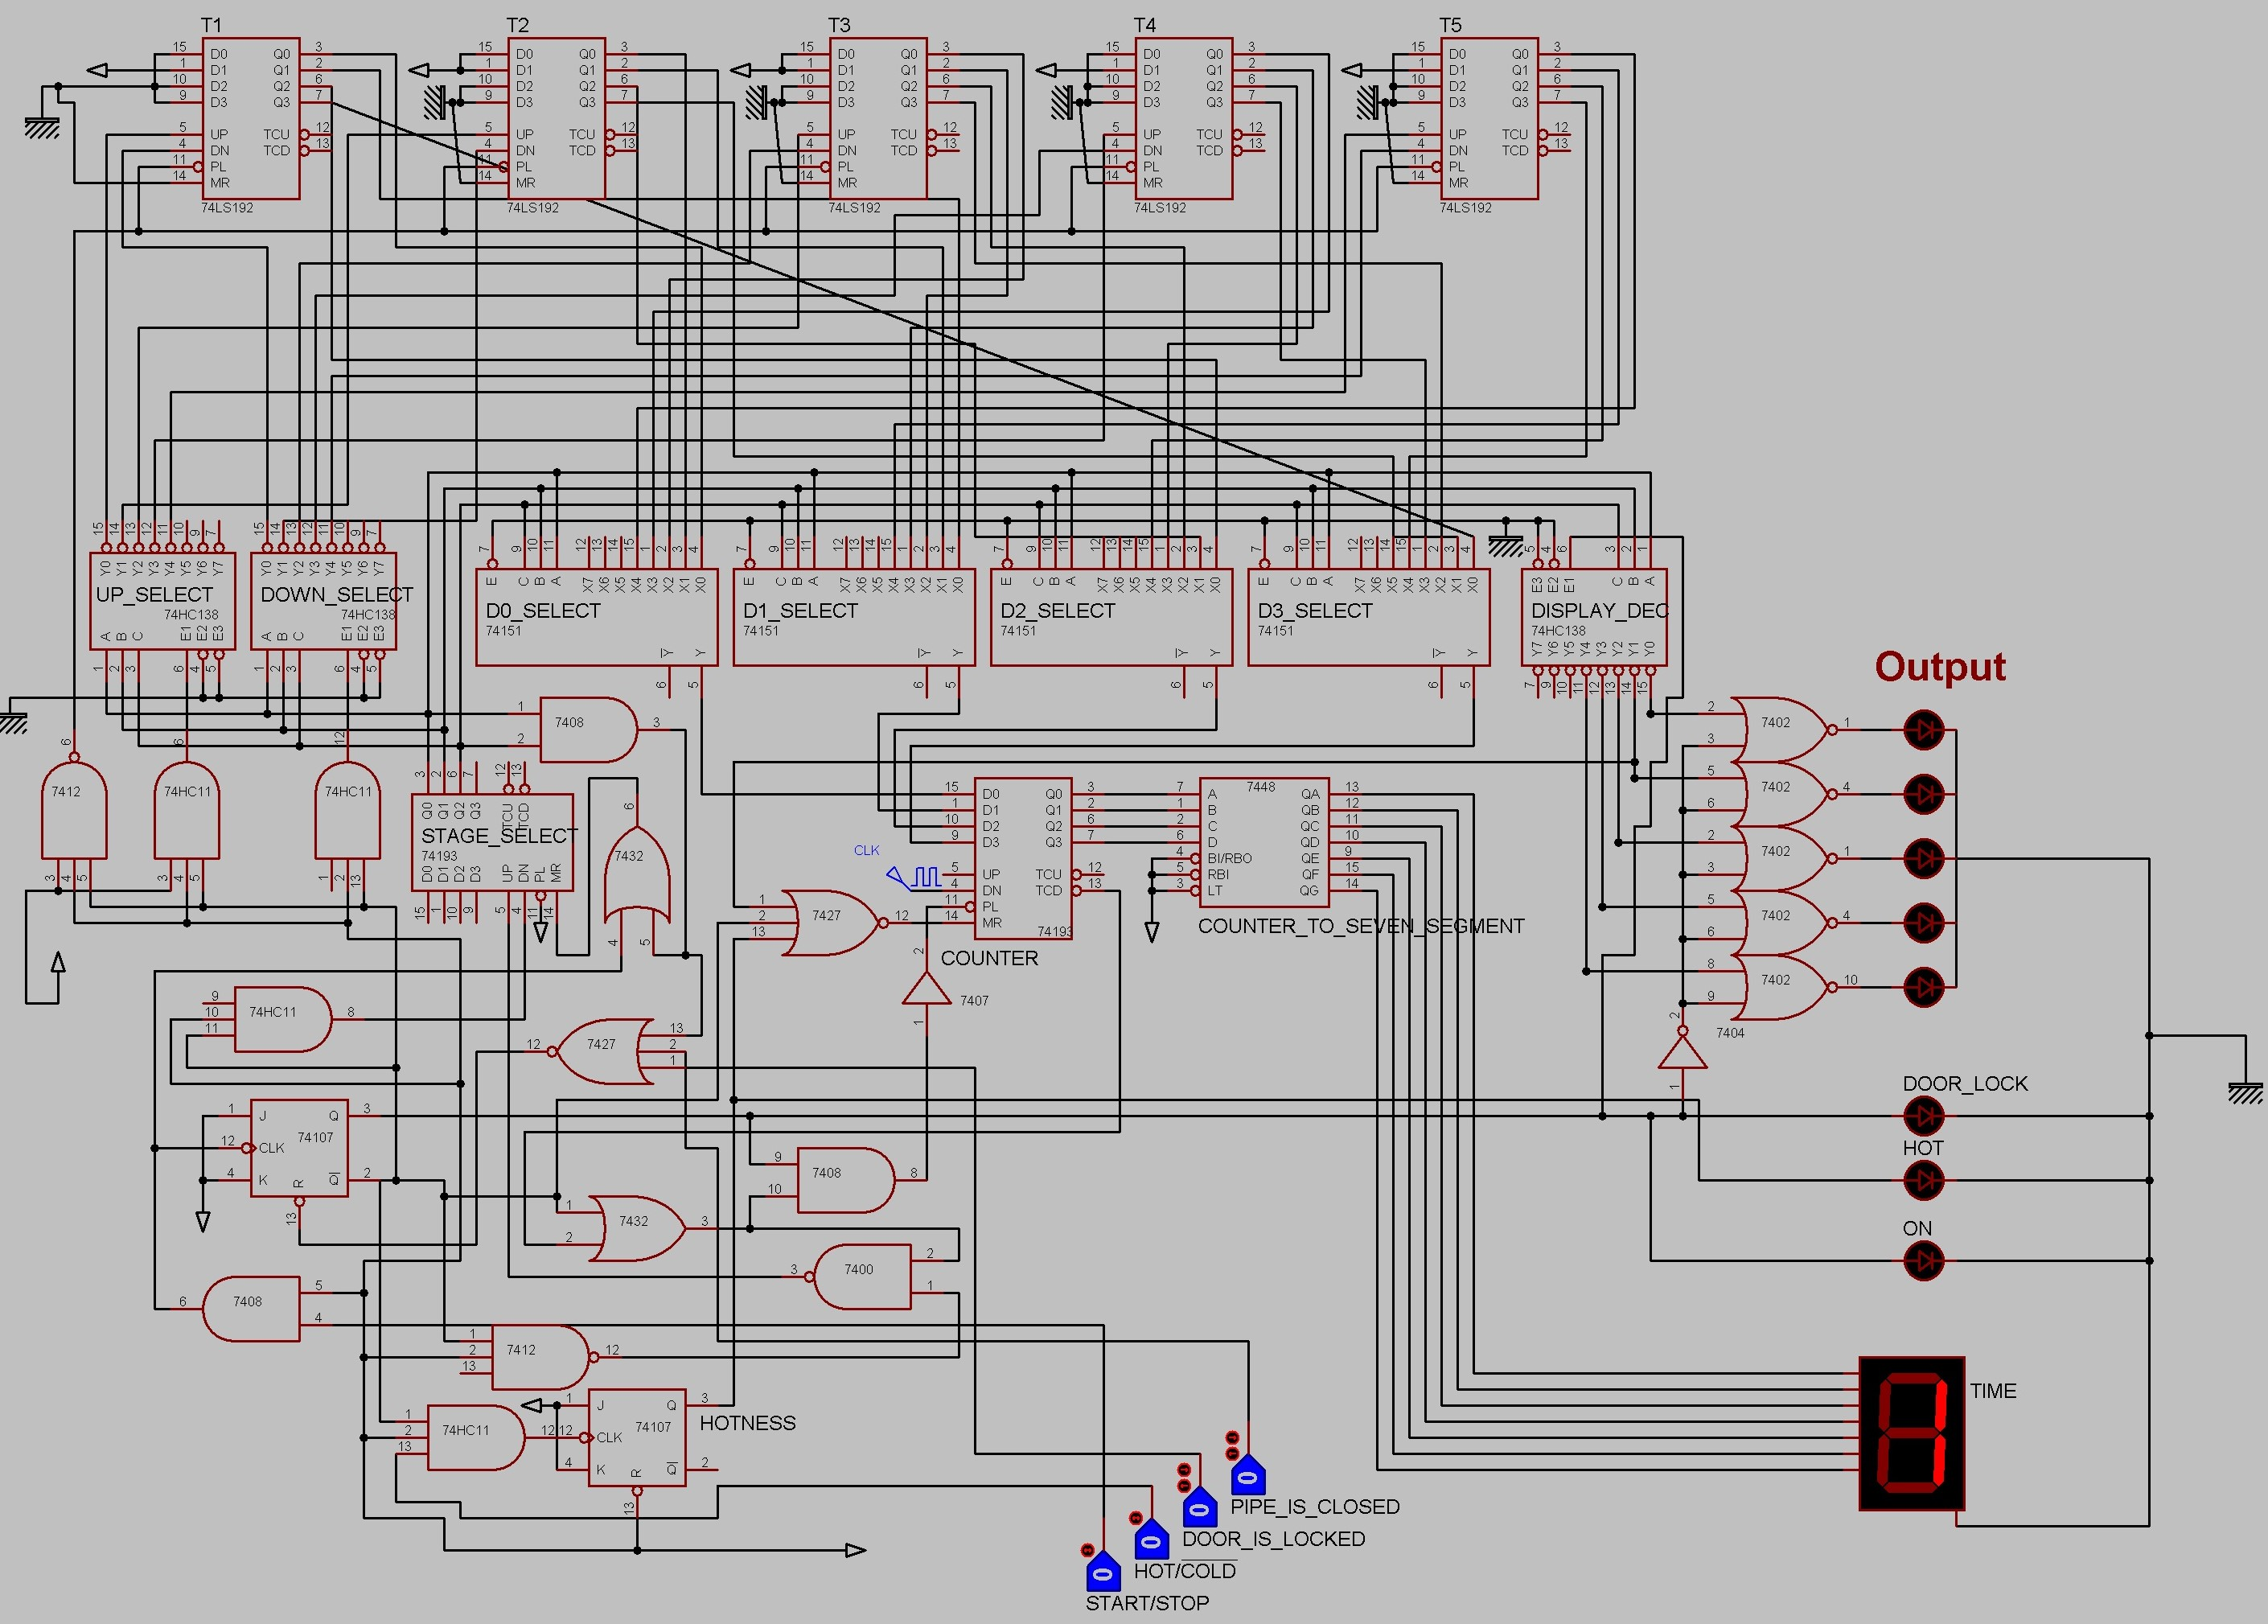
\includegraphics[scale=0.4]{madar}‎
			\caption{ جدول عملکردی تراشه 7495}
		\end{center}
	\end{figure} 
\end{document}







